% !TeX spellcheck = it_IT
\newpage
\section{Validazione}
Come facciamo a capire se una funzione di approssimazione è \textbf{buona}?
\subsection{Generalizzazione}
\begin{definition}[Generalization error]
	Misura quanto accuratamente un modello fa le predizioni su nuovi dati. Un errore basso vuol dire modello molto accurato e viceversa.
\end{definition}
La generalizzazione si basa sull'\textbf{ipotesi induttiva di generalizzazione}, secondo la quale qualunque $h$ che approssimi bene $f$ sugli esempi di training, approssimerà bene anche su dati mai visti.\\
Non è però sempre detto che sia vero e va verificato quindi nelle applicazioni. Per questo la creazione di un modello si divide in:
\begin{itemize}
	\item Fase di \textbf{apprendimento}: \textit{training} e \textit{fitting} basati sui \textit{training data}
	\item Fase \textbf{predittiva} (test): si applica il modello a nuovi esempi e si valutano le capacità di generalizzazione
\end{itemize}
\subsection{Obiettivi}
La validazione ha due obiettivi: \textbf{model selection} e \textbf{model assess}.
\begin{definition}[Model selection]
	Stimare le performance (\textit{generalization error}) di differenti modelli di apprendimento per scegliere il migliore a generalizzare. Questo implica la ricerca dei migliori iper-parametri del modello. Restituisce un modello.
\end{definition}
\begin{definition}[Model assessment]
	Una volta scelto un modello, si stima il suo errore (\textit{generalization error}) e valuta il suo rischio su un nuovo insieme di dati per il \textit{test}. Restituisce una stima.
\end{definition}
È fondamentale mantenere separati i due obiettivi e utilizzare insiemi di dati diversi.

\subsection{Hold out}
Se l'insieme dei dati è sufficientemente grande, si può dividere in tre sezioni:
\begin{itemize}
	\item \textbf{Training set}: utilizzato per l'addestramento
	\item \textbf{Validation set}: utilizzato per il \textbf{model selection}
	\item \textbf{Test set}: utilizzato per il \textbf{model assessment}
\end{itemize}
\begin{center}
	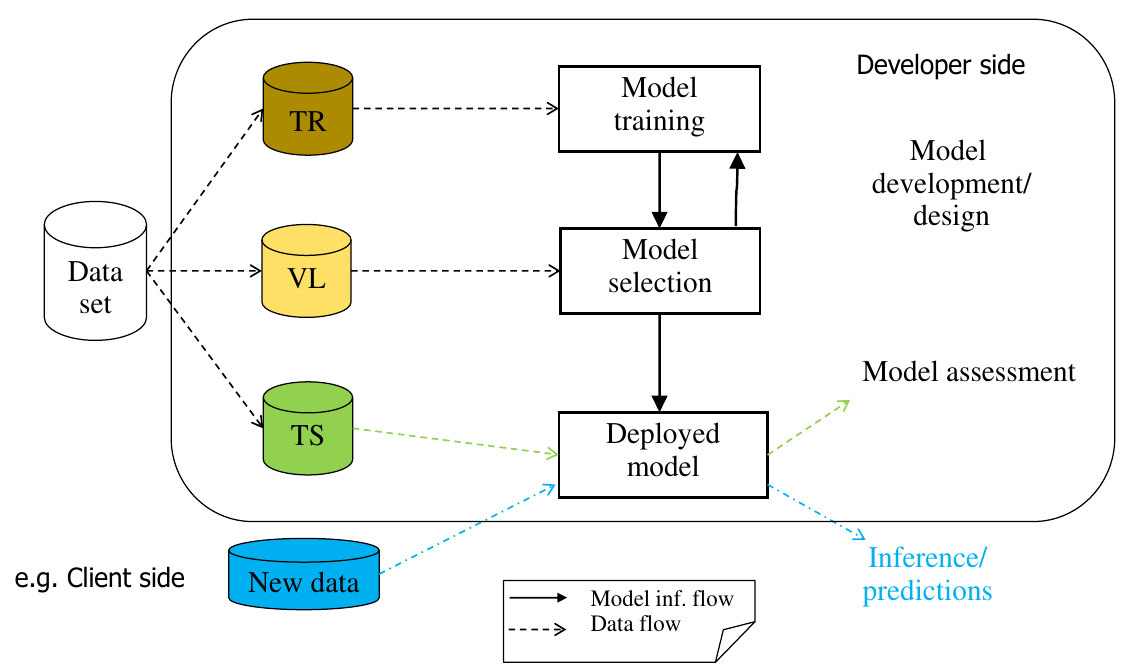
\includegraphics[scale=0.25]{validation_sets.png}
\end{center}
\begin{note}
	La stima effettuata nel \textit{model selection} non è adatta per il \textit{model assessment}.
\end{note}
\begin{note}
	I risultati del \textit{test set} non possono essere usati per il \textit{model selection}.
\end{note}
\begin{observation}
	Non possiamo utilizzare \textit{test set} in maniera ciclica, poiché falseremmo la stima del \textit{generalization error}, che restituirebbe un valore troppo ottimista.
\end{observation}
\subsubsection{Algoritmo}
Un esempio di algoritmo potrebbe seguire questi passi:
\begin{enumerate}
	\item Separazione dei dati nei tre set
	\item Si cerca la migliore $h_{w,\lambda}()$ modificando gli iper-parametri $\lambda$ del modello
	\item Per ogni valore di $\lambda$, si cerca la migliore $h_{w,\lambda}()$ che minimizzi l'errore nel \textit{TR} set, trovando i migliori parametri $w$
	\item Si seleziona la migliore $h_{w,\lambda}()$ che abbia l'errore minimo sul \textit{VL} set
	\item Opzionalmente, si può eseguire il fit di $h_{w,\lambda}()$ anche su $TR+VL$ con il miglior modello $\lambda$ 
	\item Si valuta $h_{w,\lambda}()$ sul \textit{TS} set
\end{enumerate}
Si noti che il punto 3 può essere un doppio ciclo: il primo su una griglia di valori,  per ogni $\lambda$ si addestra un modello $h_{w,\lambda}()$ e poi si calcola l'accuratezza sul \textit{VL} set. Alla fin si prende il miglior valore di $\lambda$ per errore minimo o accuratezza massima.
\begin{table}[H]
	\centering
	\begin{tabular}{|c|c|c|c|}
		\hline
		\textbf{Iper-param} & $\lambda=0.1$ & $\lambda=0.01$ & $\lambda=0.001$ \\
		\hline
		Grado 1 & Ris1 & Ris4 & Ris7 \\
		\hline
		Grado 1 & Ris2& Ris5 & Ris8 \\
		\hline
		Grado 1 & Ris3 & Ris6 & Ris9 \\
		\hline
	\end{tabular}
\end{table}

\begin{example}[Controesempio]
	Vediamo un controesempio che ci fa capire perché è necessario separare i dati. Supponiamo di avere circa $30$ esempi e $1000$ variabili di input random con target $0$ o $1$.\\
	Scelgo un modello con una sola feature che per caso indovina al $99\%$ sul dataset e su tutte le successive divisioni. Avremmo un'accuratezza del $99\%$ quando in realtà è del $50\%$.
	%TODO Non troppo chiaro, vedi la lezione
\end{example}

\subsection{K-fold}
Un'alternativa per la validazione è quella del K-fold, che prevede:
\begin{enumerate}
	\item Dividere il dataset $D$ in $k$ sottoinsiemi mutualmente esclusivi
	\item Usare l'algoritmo di addestramento sull'insieme $D\ D_i$ e testarlo su $D_i$
	\item Riassumere facendo la media di tutti i risultati $D_i$ (la diagonale)
\end{enumerate}
\begin{center}
	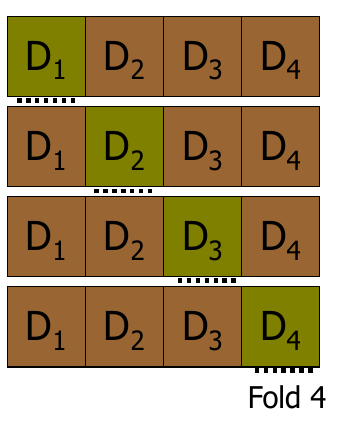
\includegraphics[scale=0.3]{kfold.png}
\end{center}
In questo modo, a differenza della tecnica \textit{Hold Out}, utilizziamo tutti i dati sia per l'addestramento che per la validazione. La problematica, oltre nel decidere il parametro $k$, sta nella complessità computazionale.

\begin{example}
	Supponiamo di dividere il dataset in \textit{Training Set} e \textit{Test Set}.
	Per effettuare la \textbf{model selection} usiamo il K-Fold sul training set, ottenendo un nuovo Training Set e Validation Set ad ogni divisione. Questo poi ci permette di trovare i migliori iper-parametri applicando una \textit{grid search}.\\
	Si addestra poi sull'intero training set e si valuta sul \textit{Test Set}.
\end{example}

\section{Complessità}
\subsection{Statistical Learning Theory}
Combinando \textit{generalizzazione}, complessità del modello e numero dei dati, otteniamo una teoria che li copre tutti.\\
L'obiettivo è di approssimare una funzione $f(x)$ con una $d$ del tipo
\begin{equation*}
	d=true\: f + noise
\end{equation*}
minimizzando la funzione di rischio
\begin{equation*}
	R = \int L(d,h(\mathbf{x}))dP(\mathbf{x},d)
\end{equation*}
dati:
\begin{itemize}
	\item Un valore $d$ e la distribuzione di probabilità $P(\mathbf{x},d)$
	\item Una funzione \textit{Loss}, ad esempio $L(h(\mathbf{x}),d)=(d-h(\mathbf{x}))^2$
\end{itemize}
\subsubsection{Empirical Risk Minimization}
Cerchiamo $h$ in $H$ che minimizzi $R$. Per farlo, dato che abbiamo un \textit{Training Set} finito, minimizziamo il \textbf{rischio empirico} (training error), trovando i migliori valori per i parametri liberi.
\begin{equation}
	R_{emp}=\frac{1}{l}\sum_{p=1}^{l}(d_p - h(\mathbf{x}_p))^2
\end{equation}
\subsubsection{Vapnik-Chervonenkis-dim}
Data $VC-dim$, una misura della complessità di $H$ (la sua flessibilità a fittare i dati), si definisce con probabilità $1-\delta$ il confine:
\begin{equation}
	R \leq R_{emp} + \epsilon (\frac{1}{l},VC, \frac{1}{\epsilon})
\end{equation}
Questo considerato che:
\begin{itemize}
	\item $\epsilon$ è una funzione che cresce con $VC$ e decresce con $l$ e $\delta$ grandi. Ovvero più dati abbiamo $>l$ e minore fiducia abbiamo sui confini di $R$.
	\item $R_{emp}$ decresce con l'aumentare della complessità del modello. Quindi un modello troppo semplice non va bene (\textbf{underfitting}).
	\item $\delta$ è la fiducia, regola la probabilità che i confini resistano. All'aumentare di $VC$, $R_{emp}$ decresce e $R$ aumenta, causando \textbf{overfitting}.
\end{itemize}
\begin{center}
	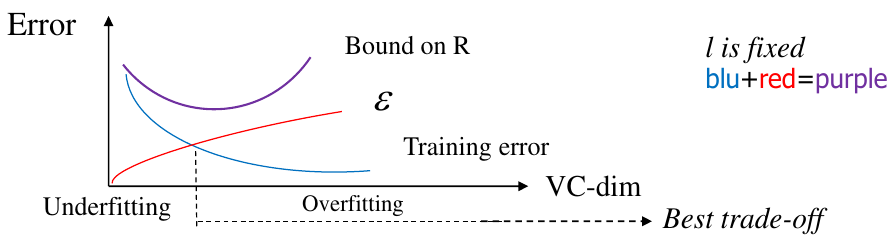
\includegraphics[scale=0.4]{slt.png}
\end{center}